\chapter{Producto}

En el capítulo anterior estudiamos la adición como una operación entre números. También vimos que una suma con varios sumandos no constituye una operación nueva: seguimos aplicando la misma operación binaria repetidas veces.

Considere, por ejemplo,
\[
2+2+2+2
\]
Podemos evaluarla sumando de a dos:
\[
(2+2)+(2+2)=4+4=8
\]
En esta expresión aparece algo particular: estamos sumando varias veces el mismo número. Naturalmente, no necesitamos una operación nueva para hallar el resultado: podríamos continuar sumando tantas veces como fuera necesario. Sin embargo, en muchos problemas interesa no sólo el total obtenido, sino también la relación entre la cantidad que se repite y el número de veces que se repite.

Por ejemplo, si una superficie requiere \(2\) litros de pintura por mano y queremos aplicar \(3\) manos, la cantidad total de pintura puede calcularse mediante
\[
2+2+2=6
\]
Aquí intervienen dos cantidades con significados distintos: \(2\) litros por mano y \(3\) manos. Del mismo modo, si un rectángulo contiene \(4\) filas de \(5\) baldosas cada una, podríamos contar sus baldosas escribiendo
\[
5+5+5+5=20
\]
En ambos casos aparece la misma estructura: una cantidad se toma cierto número de veces.

Situaciones de este tipo aparecen constantemente al medir, contar y comparar cantidades. Por ello resulta útil disponer de una operación que permita expresar directamente esta relación, sin tener que desarrollar cada vez la suma correspondiente.

Esa operación es el \emph{producto}.

\begin{example}\label{ej_intro_producto}
Considere nuevamente
\[
2+2+2+2
\]
El número \(2\) aparece como sumando cuatro veces. Esta expresión puede escribirse de manera abreviada como
\[
4\cdot2
\]
Por lo tanto,
\[
4\cdot2
=
2+2+2+2
=
8
\]
Las expresiones
\[
4\cdot2,\qquad
2+2+2+2
\qquad\text{y}\qquad
8
\]
representan el mismo número natural, aunque lo hacen de maneras diferentes.
\end{example}

\section{El producto de números naturales}

Al igual que la adición, el producto es una operación binaria: cada vez que se aplica recibe dos números.

Sobre los números naturales podemos representarlo mediante
\[
\cdot\colon\mathbb{N}\times\mathbb{N}\to\mathbb{N}
\]
Dados dos números naturales \(a\) y \(b\), escribimos su producto como
\[
a\cdot b
\]
Los números \(a\) y \(b\) reciben el nombre de \emph{factores}.
Cuando \(a\) es un número natural, la expresión
\[
a\cdot b
\]
puede interpretarse como una suma en la que \(b\) aparece \(a\) veces:
\[
a\cdot b
=
\underbrace{b+b+\cdots+b}_{a\text{ veces}}
\]
Por ejemplo,
\[
3\cdot5
=
5+5+5
=
15
\]
mientras que
\[
4\cdot2
=
2+2+2+2
=
8
\]

Esta interpretación nos permite comprender inicialmente el producto utilizando una operación que ya conocemos: la adición.

\begin{note}
La interpretación del producto como suma repetida resulta especialmente útil cuando trabajamos con números naturales.

Más adelante ampliaremos el producto a otros conjuntos numéricos. Allí encontraremos expresiones como
\[
\frac12\cdot\frac34
\]
para las cuales ya no tendría sentido hablar literalmente de ``sumar una cantidad media vez''.

Por esta razón, la suma repetida debe entenderse como una forma de construir y comprender inicialmente el producto sobre los números naturales, no como una descripción suficiente de todos los productos que estudiaremos.
\end{note}

\subsection{Producto y factores}

En una suma como
\[
3+5
\]
los números \(3\) y \(5\) reciben el nombre de \emph{sumandos}.
En un producto como
\[
3\cdot5
\]
los números \(3\) y \(5\) reciben el nombre de \emph{factores}.

El valor de la expresión completa recibe el nombre de \emph{producto}. Así,
\[
3\cdot5=15
\]

De la misma manera que una suma puede aparecer como parte de una expresión mayor, un producto también puede constituir solamente una parte de ella.
Por ejemplo, en
\[
7+3\cdot5
\]
tenemos una suma formada por dos términos:
\[
7
\qquad\text{y}\qquad
3\cdot5
\]
Dentro del segundo término aparece, a su vez, un producto cuyos factores son
\[
3
\qquad\text{y}\qquad
5.
\]
Por lo tanto, conviene distinguir el nivel de la expresión que estamos observando:
\[
\underbrace{7}_{\text{sumando}}
+
\underbrace{\left(
  \underbrace{3}_{\text{factor}}
  \cdot
  \underbrace{5}_{\text{factor}}
\right)}_{\text{sumando}}
\]
El producto completo \(3\cdot5\) es uno de los sumandos de la suma exterior. Los números \(3\) y \(5\), en cambio, son factores de ese producto.

\subsection{Una convención para evitar demasiados paréntesis}

Si quisiéramos mostrar explícitamente la estructura de
\[
7+3\cdot5
\]
podríamos escribir
\[
7+(3\cdot5)
\]
Sin embargo, utilizar paréntesis continuamente haría muchas expresiones innecesariamente difíciles de leer.

Por convenio, cuando aparecen productos y sumas en una misma expresión, los productos se consideran agrupados antes que las sumas. Así,
\[
7+3\cdot5
\]
se interpreta como
\[
7+(3\cdot5)
\]
y no como
\[
(7+3)\cdot5
\]
Esta convención recibe el nombre de \emph{precedencia} o \emph{jerarquía de las operaciones}.

No significa que el producto sea una operación ``más importante'' que la suma. Es simplemente una regla de escritura que permite reconocer sin ambigüedad cuáles son los términos de una expresión.

Por ejemplo, en
\[
2+4\cdot3+5
\]
los términos de la suma son
\[
2,\qquad4\cdot3,\qquad5
\]
Si evaluamos el producto,
\[
4\cdot3=12
\]
la expresión queda
\[
2+12+5
\]
Ahora resulta evidente que estamos ante una suma cuyos sumandos son
\[
2,\qquad12,\qquad5
\]
Por lo tanto,
\[
2+4\cdot3+5
=
2+12+5
=
19
\]

\section{Propiedades del producto}

Hemos introducido el producto de números naturales mediante sumas repetidas. Esto nos permite hacer algo importante: muchas de sus propiedades pueden comprenderse utilizando únicamente ideas que ya conocemos sobre la adición.

No se trata de memorizar una nueva colección de reglas independientes. En muchos casos podremos desarmar un producto en sumas, utilizar las propiedades de la adición y volver a escribir el resultado como un producto.

\subsection{Clausura}

Como el producto entre números naturales puede construirse mediante sumas de números naturales, su resultado vuelve a ser un número natural.

Por ejemplo,
\[
4\cdot3
=
3+3+3+3
=
12
\]
y
\[
12\in\mathbb{N}
\]
De manera general, si
\[
a,b\in\mathbb{N}
\]
entonces
\[
a\cdot b\in\mathbb{N}
\]
Por eso decimos que los números naturales son \emph{cerrados} respecto del producto.

\subsection{Propiedad conmutativa}

Considere
\[
3\cdot4
\]
Según nuestra interpretación del producto,
\[
3\cdot4
=
4+4+4
=
12.
\]
En cambio,
\[
4\cdot3
=
3+3+3+3
=
12.
\]
En ambos casos obtenemos el mismo número:
\[
3\cdot4=4\cdot3
\]
Este hecho puede comprenderse de una manera sencilla si imaginamos una disposición rectangular de objetos. El producto
\[
3\cdot4
\]
puede representar tres filas de cuatro objetos:
\[
\begin{array}{cccc}
\bullet&\bullet&\bullet&\bullet\\
\bullet&\bullet&\bullet&\bullet\\
\bullet&\bullet&\bullet&\bullet
\end{array}
\]
Pero esa misma disposición también puede observarse como cuatro columnas de tres objetos. Contar por filas o contar por columnas no modifica la cantidad de objetos.
De manera general,
\[
a\cdot b=b\cdot a
\]
Esta propiedad recibe el nombre de \emph{propiedad conmutativa del producto}.
Gracias a ella, aunque inicialmente interpretemos
\[
a\cdot b
\]
como \(a\) repeticiones de \(b\), también podemos interpretarlo como \(b\) repeticiones de \(a\).

\subsection{Elemento neutro}

Considere ahora el producto
\[
1\cdot a
\]
Según la interpretación de suma repetida, esto significa tomar una sola vez el número \(a\). Por lo tanto,
\[
1\cdot a=a
\]
Como el producto es conmutativo,
\[
a\cdot1=1\cdot a=a
\]
Así,
\[
a\cdot1=1\cdot a=a
\]
El número \(1\) recibe el nombre de \emph{elemento neutro del producto}: multiplicar un número por \(1\) no modifica la cantidad representada.

\subsection{Producto por cero}

Veamos ahora qué ocurre con el número \(0\).

La expresión
\[
a\cdot0
\]
representa la suma de \(a\) ceros:
\[
\underbrace{0+0+\cdots+0}_{a\text{ veces}}
\]
Como sumar ceros no modifica la cantidad,
\[
a\cdot0=0
\]
Por la propiedad conmutativa,
\[
0\cdot a=a\cdot0=0
\]
Por lo tanto,
\[
a\cdot0=0\cdot a=0
\]
El cero no es un elemento neutro del producto. Por el contrario, cualquier producto que tenga al \(0\) como factor representa el número \(0\).

\subsection{Propiedad asociativa}

El producto, al igual que la suma, es una operación binaria. Por esta razón, una expresión como
\[
2\cdot3\cdot4
\]
representa aplicaciones sucesivas del producto.
Podríamos agrupar primero
\[
2\cdot3
\]
y escribir
\[
(2\cdot3)\cdot4
\]
Como
\[
2\cdot3=6
\]
obtenemos
\[
6\cdot4=24
\]
Pero también podríamos comenzar por
\[
3\cdot4
\]
y escribir
\[
2\cdot(3\cdot4)
\]
Como
\[
3\cdot4=12
\]
obtenemos
\[
2\cdot12=24
\]
Ambas formas de agrupar representan el mismo número:
\[
(2\cdot3)\cdot4
=
2\cdot(3\cdot4)
\]
Podemos comprender por qué ocurre esto utilizando nuevamente la suma repetida.
La expresión
\[
a\cdot(b\cdot c)
\]
significa tomar \(a\) veces la cantidad \(b\cdot c\):
\[
\underbrace{(b\cdot c)+(b\cdot c)+\cdots+(b\cdot c)}_{a\text{ veces}}
\]
Pero cada \(b\cdot c\) representa, a su vez,
\[
\underbrace{c+c+\cdots+c}_{b\text{ veces}}
\]
Por lo tanto, en total estamos sumando \(c\) una cantidad de \(a\cdot b\) veces. Esto puede escribirse como
\[
(a\cdot b)\cdot c
\]
Así obtenemos, de manera general,
\[
(a\cdot b)\cdot c
=
a\cdot(b\cdot c)
\]
Esta es la \emph{propiedad asociativa del producto}.
Gracias a ella podemos escribir simplemente
\[
a\cdot b\cdot c
\]
sin indicar mediante paréntesis qué producto debe realizarse primero, siempre que en la expresión intervengan únicamente productos.

\subsection{Propiedad distributiva}

Existe además una propiedad especialmente importante porque relaciona las dos operaciones que conocemos hasta ahora: la suma y el producto.

Considere
\[
3\cdot(2+4)
\]
Como el primer factor indica cuántas veces repetimos el segundo,
\[
3\cdot(2+4)
=
(2+4)+(2+4)+(2+5)
\]
Utilizando las propiedades asociativa y conmutativa de la adición podemos reorganizar los sumandos:
\[
(2+2+2)+(4+4+4)
\]
Ahora reconocemos nuevamente dos productos:
\[
2+2+2=3\cdot2
\]
y
\[
4+4+4=3\cdot4
\]
Por lo tanto,
\[
3\cdot(2+4)
=
3\cdot2+3\cdot4
\]
De manera general,
\[
a\cdot(b+c)
=
a\cdot b+a\cdot c
\]
Esta propiedad recibe el nombre de \emph{propiedad distributiva del producto respecto de la suma}.

También podemos encontrar la suma en el primer factor. Por ejemplo,
\[
(2+3)\cdot4
\]
Según la interpretación del producto, estamos sumando \(4\) un total de \(2+3\) veces:
\[
\underbrace{4+4}_{2\text{ veces}}
+
\underbrace{4+4+4}_{3\text{ veces}}
\]
Podemos reconocer entonces
\[
2\cdot4+3\cdot4
\]
Por lo tanto,
\[
(a+b)\cdot c
=
a\cdot c+b\cdot c
\]
Ambas formas expresan la misma idea:
\begin{gather*}
a\cdot(b+c)=a\cdot b+a\cdot c \\
(a+b)\cdot c=a\cdot c+b\cdot c
\end{gather*}
La propiedad distributiva será especialmente importante porque permite transformar expresiones que contienen productos y sumas sin modificar el número que representan.

\subsection{¿Qué hemos obtenido a partir de la suma?}

Resulta útil observar lo que acabamos de hacer.

Partimos de una interpretación muy sencilla:
\[
a\cdot b
=
\underbrace{b+b+\cdots+b}_{a\text{ veces}}
\]
A partir de ella pudimos comprender varias propiedades del producto:
\begin{gather*}
  a\cdot b=b\cdot a,\\
  (a\cdot b)\cdot c=a\cdot(b\cdot c),\\
  a\cdot1=a,\\
  a\cdot0=0,
\end{gather*}
y
\[
a\cdot(b+c)=a\cdot b+a\cdot c.
\]
Esto muestra que la relación entre suma y producto es más profunda que una simple abreviatura de escritura. Sobre los números naturales, el producto puede construirse a partir de sumas repetidas y gran parte de su comportamiento puede comprenderse utilizando las propiedades que ya conocemos de la adición.

Sin embargo, suma y producto continúan siendo operaciones diferentes. En una expresión es importante reconocer cuál de ellas está actuando en cada nivel.

Por ejemplo, en
\[
2+3\cdot4+5
\]
los sumandos de la expresión principal son
\[
2,\qquad3\cdot4,\qquad5,
\]
mientras que \(3\) y \(4\) son los factores del producto
\[
3\cdot4
\]
Esta distinción será fundamental para interpretar correctamente expresiones que combinen varias operaciones.


\section[Práctica inicial con productos]{Práctica inicial con productos de números naturales}

Antes de ampliar el producto a otros conjuntos numéricos, conviene practicar las ideas más elementales que acabamos de introducir. En estos ejercicios no buscamos todavía trabajar con cálculos complicados, sino reconocer distintas formas de representar un mismo número y distinguir la estructura de las expresiones.

\subsection*{De sumas repetidas a productos}

Escriba cada suma repetida como un producto. No es necesario evaluarlo en un primer paso.

\begin{enumerate}
\item \(3+3+3\)
\item \(5+5+5+5\)
\item \(2+2+2+2+2+2\)
\item \(7+7\)
\item \(10+10+10\)
\item \(1+1+1+1+1\)
\end{enumerate}

Por ejemplo,
\[
4+4+4=3\cdot4.
\]
Observe que el primer factor indica cuántas veces aparece el segundo como sumando.

\subsection*{De productos a sumas repetidas}

Realice ahora el proceso contrario. Escriba cada producto como una suma repetida y luego encuentre un único numeral que represente su valor.

\begin{enumerate}
\item \(2\cdot3\)
\item \(4\cdot2\)
\item \(3\cdot5\)
\item \(5\cdot4\)
\item \(2\cdot10\)
\item \(6\cdot1\)
\end{enumerate}

\subsection*{Evaluar productos}

Encuentre un único numeral que represente el valor de cada expresión.

\begin{enumerate}
\item \(3\cdot4\)
\item \(6\cdot2\)
\item \(5\cdot5\)
\item \(7\cdot3\)
\item \(8\cdot1\)
\item \(9\cdot0\)
\item \(2\cdot4\cdot3\)
\item \(5+2\cdot3\)
\item \(4\cdot2+7\)
\item \(2+3\cdot4+1\)
\end{enumerate}

Recuerde que, cuando aparecen sumas y productos en una misma expresión, el producto se considera agrupado antes que la suma.

\subsection*{Completar expresiones equivalentes}

Complete los espacios de manera que ambos lados de cada igualdad representen el mismo número natural.

\begin{enumerate}
\item \(3\cdot4=\square\)
\item \(5+5+5=\square\cdot5\)
\item \(4\cdot3=3\cdot\square\)
\item \(7\cdot1=\square\)
\item \(9\cdot0=\square\)
\item \(2\cdot(3+4)=2\cdot3+2\cdot\square\)
\end{enumerate}

\subsection*{Reconocer la estructura de una expresión}

En cada caso, indique cuál es la operación principal. Si la expresión principal es una suma, identifique sus sumandos; si contiene productos, identifique también los factores de cada producto.

\begin{enumerate}
\item \(3\cdot5\)
\item \(7+2\cdot4\)
\item \(3\cdot2+5\)
\item \(2+4\cdot3+1\)
\item \(5\cdot(2+3)\)
\item \((2+3)\cdot4\)
\end{enumerate}

El objetivo de estos ejercicios no es únicamente obtener resultados. También debe poder reconocer qué operación está actuando en cada nivel de una expresión y qué papel cumple cada número dentro de ella.

\section{El producto de números enteros}

La interpretación del producto como suma repetida nos permitió construir el producto de números naturales. Sin embargo, ya no basta para explicar expresiones como
\[
(-3)\cdot4,
\qquad
3\cdot(-4)
\qquad\text{o}\qquad
(-3)\cdot(-4).
\]
No tiene sentido interpretar literalmente la primera de ellas como ``sumar \(4\) menos tres veces''. Necesitamos extender el producto a los números enteros.

Al hacerlo, no abandonaremos las propiedades que ya conocemos: el producto seguirá siendo asociativo y conmutativo, tendrá al \(1\) como elemento neutro, se distribuirá respecto de la suma y continuará cumpliendo que el producto por cero es cero. Estas propiedades permitirán determinar qué debe significar multiplicar por un número negativo.

Así, el producto puede considerarse ahora como una operación
\[
\cdot\colon\mathbb{Z}\times\mathbb{Z}\to\mathbb{Z}.
\]
En particular, el producto de dos enteros vuelve a ser un entero.

\subsection{El opuesto como producto por \texorpdfstring{\(-1\)}{-1}}

Recordemos que \(-1\) es el opuesto de \(1\). Por lo tanto,
\[
(-1)+1=0
\]
Multipliquemos ambos sumandos por un entero \(a\). Por la propiedad distributiva,
\begin{gather*}
a\cdot\bigl((-1)+1\bigr)
=a\cdot(-1)+a\cdot1
\end{gather*}
Operando usando las propiedades, obtenemos
\begin{align*}
  a\cdot\bigl((-1)+1\bigr) &= a\cdot(-1)+a\cdot 1 \\ 
  a \cdot (0) &= a\cdot(-1) + a\cdot1 \\ 
  0 &= a\cdot(-1) + a \\ 
  -a + 0 &= a\cdot(-1) +a - a \\ 
  -a &= a\cdot(-1)
\end{align*}
Es decir, \(a\cdot(-1)\) es el opuesto de \(a\). Por la definición de opuesto,
\[
\boxed{a\cdot(-1)=-a}
\]
Esta igualdad conecta el producto con la idea estudiada en el capítulo anterior: un entero negativo puede escribirse como el producto de su opuesto positivo por \(-1\).

\subsection{Producto por un opuesto}

Si \(b\) es un entero, acabamos de ver que
\[
-b=b\cdot(-1)
\]
Entonces, usando la propiedad asociativa,
\begin{align*}
a\cdot(-b)
&=a\cdot\bigl(b\cdot(-1)\bigr)\\
&=(a\cdot b)\cdot(-1)\\
&=-(a\cdot b)
\end{align*}
Por la propiedad conmutativa se obtiene también
\[
(-a)\cdot b=-(a\cdot b)
\]
Por lo tanto, multiplicar exactamente uno de los factores por su opuesto produce el opuesto del producto.

\subsection{Producto de dos opuestos}

Ahora podemos determinar el producto de dos números negativos sin memorizar una regla nueva. Como \(-a=a\cdot(-1)\), tenemos
\begin{align*}
(-a)\cdot(-b)
&=\bigl(a\cdot(-1)\bigr)\cdot(-b)\\
&=(-1)\cdot\bigl(a\cdot(-b)\bigr)
\end{align*}
En la segunda igualdad usamos las propiedades asociativa y conmutativa. Por la sección anterior,
\[
a\cdot(-b)=-(a\cdot b)
\]
Por consiguiente,
\begin{align*}
(-a)\cdot(-b)
&=(-1)\cdot\bigl(-(a\cdot b)\bigr)\\
&=-\bigl(-(a\cdot b)\bigr)\\
&=a\cdot b
\end{align*}
Así, el producto de dos opuestos es el producto de los números originales:
\[
\boxed{(-a)\cdot(-b)=a\cdot b}
\]

Las cuatro posibilidades para los signos se resumen ahora en consecuencias de los opuestos:
\begin{gather*}
(+a)\cdot(+b)=a\cdot b\\
(-a)\cdot(+b)=-(a\cdot b)\\
(+a)\cdot(-b)=-(a\cdot b)\\
(-a)\cdot(-b)=a\cdot b
\end{gather*}
Por ejemplo,
\[
(-3)\cdot(-4)=3\cdot4=12
\]

\section{Números racionales}

El producto de enteros funciona para cualesquiera dos enteros. Sin embargo, todavía existen ecuaciones que no pueden resolverse dentro de \(\mathbb{Z}\). Considere, por ejemplo,
\[
2\cdot x=1
\]
No existe ningún entero que, multiplicado por \(2\), produzca \(1\).

Esta dificultad es análoga a la que apareció anteriormente con expresiones como
\[
3-7
\]
Allí fue necesario ampliar los números naturales para introducir los enteros. Ahora necesitamos una nueva ampliación que permita representar números capaces de resolver ecuaciones como \(2\cdot x=1\).

\subsection{Fracciones}

Sean \(a,b\in\mathbb{Z}\) con \(b\ne0\). Introducimos la escritura
\[
\begin{tikzpicture}[baseline=(frac.base),>=stealth]
  \node (frac) {\(\displaystyle \frac{a}{b}\)};

  \node[right=.5cm of frac, yshift=0.2cm ,font=\footnotesize] (num) {Numerador};
  \node[right=.5cm of frac, yshift=-0.2cm,font=\footnotesize] (den) {Denominador};

  \draw[->] (num.west) -- ([yshift=0.2cm]frac.east);
  \draw[->] (den.west) -- ([yshift=-0.2cm]frac.east);
\end{tikzpicture}
\]
para representar el número que satisface
\[
b\cdot\frac{a}{b}=a
\]
Por ejemplo,
\[
2\cdot\frac12=1
\]
de modo que \(\frac12\) resuelve precisamente la ecuación que no tenía solución en los enteros.

La expresión \(\frac{a}{b}\) recibe el nombre de \emph{fracción}. Los números que pueden representarse mediante una fracción de enteros, con denominador distinto de cero, se llaman \emph{números racionales}.

\begin{definition}[Número racional]
Un número racional es un número que puede representarse mediante una fracción
\[
\frac{a}{b}
\qquad a,b\in\mathbb{Z},\quad b\ne0
\]
El conjunto de los números racionales se representa mediante \(\mathbb{Q}\).
\end{definition}

Una misma cantidad puede tener distintas representaciones fraccionarias. Veamos primero un ejemplo.

Sabemos que
\[
2\cdot\frac12=1
\]
Es decir, \(\frac12\) es el número que satisface la ecuación
\[
2x=1
\]
Multipliquemos ahora ambos lados de esta ecuación por \(2\):
\[
4x=2
\]
La solución sigue siendo la misma. Por lo tanto, el número que representábamos como \(\frac12\) también puede representarse como
\[
\frac24
\]
Así,
\[
\frac12=\frac24
\]
Podemos hacer lo mismo multiplicando la ecuación original por \(50\):
\[
100x=50
\]
Nuevamente, la solución no ha cambiado. Por eso,
\[
\frac12=\frac{50}{100}
\]
En consecuencia,
\[
\frac12=\frac24=\frac{50}{100}
\]
El mismo razonamiento funciona en general. Si
\[
bx=a
\qquad b\ne0
\]
entonces \(x\) puede representarse mediante
\[
\frac{a}{b}
\]
Si multiplicamos ambos lados de la ecuación por un entero \(c\ne0\), obtenemos
\[
(bc)x=ac
\]
Pero \(x\) sigue siendo el mismo número. Por lo tanto, también puede representarse como
\[
\frac{ac}{bc}
\]
Así llegamos a la relación
\[
\boxed{
\frac{a}{b}
=
\frac{ac}{bc}
}
\qquad c\ne0
\]
Es decir, multiplicar el numerador y el denominador por un mismo entero distinto de cero cambia la representación de una fracción, pero no el número que representa.

Los enteros también son racionales. En efecto, para cualquier entero \(a\),
\[
1\cdot a=a
\]
de modo que \(a\) puede representarse como
\[
a=\frac{a}{1}
\]
Por lo tanto,
\[
\mathbb{Z}\subseteq\mathbb{Q}
\]

\subsection{Producto de números racionales}

Ahora extendemos el producto a los números racionales. Antes de establecer cómo se multiplican dos fracciones, conviene preguntarse qué debe representar ese producto.

Sean
\[
\frac{a}{b}
  \qquad\text{y}\qquad
  \frac{c}{d}
\]
con \(a,b,c,d\in\mathbb{Z}\), \(b\ne0\) y \(d\ne0\).

Por la forma en que hemos construido las fracciones, sabemos que
\[
b\cdot\frac{a}{b}=a
\]
y
\[
d\cdot\frac{c}{d}=c
\]
Consideremos ahora el producto
\[
\frac{a}{b}\cdot\frac{c}{d}
\]
Queremos averiguar qué número representa. Para ello, multipliquémoslo por \(b\cdot d\):
\[
(b\cdot d)\cdot
\left(
\frac{a}{b}\cdot\frac{c}{d}
\right)
\]
Usando la asociatividad y la conmutatividad del producto, podemos reorganizar los factores:
\[
(b\cdot d)\cdot
\left(
\frac{a}{b}\cdot\frac{c}{d}
\right)
=
\left(
b\cdot\frac{a}{b}
\right)
\cdot
\left(
d\cdot\frac{c}{d}
\right)
\]
Pero
\[
b\cdot\frac{a}{b}=a
\]
y
\[
d\cdot\frac{c}{d}=c
\]
Por lo tanto,
\[
(b\cdot d)\cdot
\left(
\frac{a}{b}\cdot\frac{c}{d}
\right)
=
a\cdot c
\]
Es decir, buscamos un número que, multiplicado por \(b\cdot d\), dé como resultado \(a\cdot c\). Precisamente, la fracción
\[
\frac{a\cdot c}{b\cdot d}
\]
representa ese número, pues
\[
(b\cdot d)\cdot
\frac{a\cdot c}{b\cdot d}
=
a\cdot c
\]
Así obtenemos
\[
\boxed{
\frac{a}{b}\cdot\frac{c}{d}
=
\frac{a\cdot c}{b\cdot d}
}
\]
Esta expresión no es una regla arbitraria. Los denominadores se multiplican porque \(b\cdot d\) permite eliminar simultáneamente los dos denominadores, mientras que los numeradores se multiplican porque, al hacerlo, quedan las cantidades \(a\) y \(c\), cuyo producto es \(a\cdot c\).

Veámoslo en un caso concreto:
\[
\frac23\cdot\frac34
\]
Si multiplicamos este producto por \(3\cdot4=12\), obtenemos
\[
12\cdot
\left(
\frac23\cdot\frac34
\right)
=
\left(
3\cdot\frac23
\right)
\cdot
\left(
4\cdot\frac34
\right)
\]
Como
\[
3\cdot\frac23=2
\]
y
\[
4\cdot\frac34=3
\]
resulta
\[
12\cdot
\left(
\frac23\cdot\frac34
\right)
=
2\cdot3
=
6
\]
Por lo tanto, el producto debe ser el número que multiplicado por \(12\) da \(6\):
\[
\frac23\cdot\frac34
=
\frac6{12}
=
\frac12
\]
Las relaciones de signo obtenidas para los enteros continúan siendo válidas. Por ejemplo,
\[
\frac{-2}{3}\cdot\frac34
=
-\left(
\frac23\cdot\frac34
\right)
=
-\frac12
\]

Así, la interpretación inicial del producto como suma repetida ya no es necesaria para describir todos los casos. El producto se ha extendido primero a los enteros y luego a los racionales conservando las propiedades que venimos utilizando.

\subsection{Inverso multiplicativo}

El número \(1\) es el elemento neutro del producto. Por eso resulta natural preguntar, dado un racional no nulo, qué número debemos multiplicar por él para obtener \(1\).

Sea
\[
\frac{a}{b}\ne0
\]

Como \(b\ne0\), para que la fracción sea distinta de cero debe cumplirse también
\[
a\ne0
\]

Buscamos entonces un número \(x\) que satisfaga
\[
\frac{a}{b}\cdot x=1
\]

¿Qué forma debe tener ese número?

Sabemos que, al multiplicar fracciones, los numeradores se multiplican entre sí y los denominadores también. Por lo tanto, necesitamos que los factores que aparecen en el numerador y en el denominador puedan formar dos productos iguales, ya que una fracción cuyo numerador y denominador representan el mismo número no nulo es igual a \(1\).

Consideremos la fracción
\[
\frac{b}{a}
\]

Al multiplicarla por \(\frac{a}{b}\), obtenemos
\[
\frac{a}{b}\cdot\frac{b}{a}
=
\frac{a\cdot b}{b\cdot a}
\]

Por la conmutatividad del producto,
\[
a\cdot b=b\cdot a
\]

Así, el numerador y el denominador representan el mismo número:
\[
\frac{a\cdot b}{b\cdot a}
=
\frac{a\cdot b}{a\cdot b}
=
1
\]

Por lo tanto,
\[
\frac{a}{b}\cdot\frac{b}{a}=1
\]

Esto muestra que \(\frac{b}{a}\) es precisamente el número que, multiplicado por \(\frac{a}{b}\), produce el elemento neutro del producto.

Por esta razón, llamamos \emph{inverso multiplicativo} de un número racional no nulo al número que, al multiplicarse por él, da como resultado \(1\).

En particular,
\[
\boxed{
\left(\frac{a}{b}\right)^{-1}
=
\frac{b}{a}
}
\qquad
a\ne0
\]

La expresión anterior no debe entenderse solamente como una regla para ``dar vuelta'' una fracción. El intercambio entre numerador y denominador aparece porque buscamos que, al multiplicar ambas fracciones, el numerador y el denominador del resultado sean iguales.

Por ejemplo, consideremos
\[
\frac{3}{5}
\]

Buscamos un número \(x\) tal que
\[
\frac{3}{5}\cdot x=1
\]

Si elegimos
\[
x=\frac{5}{3}
\]
entonces
\[
\frac{3}{5}\cdot\frac{5}{3}
=
\frac{3\cdot5}{5\cdot3}
=
\frac{15}{15}
=
1
\]

Por eso,
\[
\left(\frac35\right)^{-1}
=
\frac53
\]

El cero, en cambio, no posee inverso multiplicativo. Para que un número \(x\) fuera su inverso, debería cumplirse
\[
0\cdot x=1
\]

Pero ya sabemos que, para cualquier número \(x\),
\[
0\cdot x=0
\]

Por lo, no existe ningún número que multiplicado por \(0\) dé como resultado \(1\), y en consecuencia \(0\) no tiene inverso multiplicativo.

\subsection{División}

Una vez introducidos los inversos multiplicativos, podemos definir la división sin recurrir a restas repetidas.

Dados \(x,y\in\mathbb{Q}\) con \(y\ne0\), definimos
\[
\boxed{x\div y=x\cdot y^{-1}}
\]
Es decir, dividir por un número no nulo consiste en multiplicar por su inverso.

En particular,
\[
\frac{a}{b}\div\frac{c}{d}
=
\frac{a}{b}\cdot\frac{d}{c}
=
\frac{a\cdot d}{b\cdot c},
\quad c\ne0.
\]
Por ejemplo,
\[
\frac34\div\frac25
=
\frac34\cdot\frac52
=
\frac{15}{8}
\]

Esta definición también explica expresiones como
\[
1\div2=\frac12
\]
La división ya no depende de que el cociente sea un número entero.

\subsection{Restas sucesivas como estrategia de cálculo}

En algunos casos particulares, cuando dividimos números naturales y el cociente es también natural, las restas sucesivas pueden utilizarse como una estrategia de cálculo.

Por ejemplo, para evaluar
\[
12\div3
\]
podemos restar \(3\) repetidamente hasta llegar a cero:
\begin{align*}
12-3&=9\\
9-3&=6\\
6-3&=3\\
3-3&=0
\end{align*}
Se realizaron cuatro restas, por lo que
\[
12\div3=4
\]
Sin embargo, este procedimiento encuentra rápidamente una dificultad. Consideremos
\[
1\div2
\]
No podemos restar \(2\) de \(1\) y continuar obteniendo números naturales. Esto no significa que la división carezca de resultado, sino que su resultado no pertenece a \(\mathbb N\).

Ya sabemos que
\[
1\div2=\frac12
\]
Pero también podemos representar este mismo número de otra manera.

\subsection{Partes de la unidad y escritura decimal}

Nuestro sistema de numeración utiliza potencias\footnote{El término de potencia matemática se profundizará en el próximo capítulo.} de \(10\). Del mismo modo que podemos agrupar diez unidades para formar una decena, también podemos recorrer el camino contrario y dividir una unidad en diez partes iguales.

Cada una de esas partes es un \emph{décimo}:
\[
\frac{1}{10}
\]
Cinco décimos se representan mediante
\[
\frac{5}{10}
\]
Como
\begin{align*}
  \frac12&=1\cdot\frac{1}{2}\\
  &=\frac55\cdot\frac12\\ 
  &=\frac{5}{10}
\end{align*}
podemos pensar en la mitad de una unidad como cinco décimos.

La escritura decimal permite representar esos cinco décimos de la siguiente manera:
\[
0{,}5
\]
Por lo tanto,
\[
\frac12=\frac{5}{10}=0{,}5
\]
Y como
\[
1\div2=\frac12
\]
obtenemos
\[
\boxed{
1\div2=\frac12=0{,}5
}
\]
Las expresiones
\[
1\div2,\qquad \frac12,\qquad 0{,}5
\]
no representan tres números diferentes. Son distintas formas de representar el mismo número.

La coma decimal separa la parte entera de las partes de la unidad. La primera posición situada a la derecha de la coma representa décimos:
\[
0{,}1=\frac{1}{10}
\]
La segunda posición representa centésimos:
\[
0{,}01=\frac{1}{100}
\]
La tercera representa milésimos:
\[
0{,}001=\frac{1}{1000}
\]
Por ejemplo,
\[
0{,}3=\frac{3}{10}
\]
y
\[
0{,}25=\frac{25}{100}
\]
Como
\[
\frac{25}{100}=\frac14
\]
también podemos escribir
\[
\frac14=0{,}25
\]
De este modo, la escritura decimal no introduce necesariamente números nuevos. Proporciona otra representación para aquellos números racionales que pueden expresarse mediante fracciones cuyo denominador es una potencia de \(10\), o mediante una fracción equivalente de ese tipo.

Esto también permite comprender qué ocurre cuando el dividendo es menor que el divisor. En
\[
1\div2
\]
no hay ninguna unidad completa de \(2\) dentro de \(1\), pero podemos dividir la unidad en partes más pequeñas. Al expresarla como diez décimos,
\[
1=\frac{10}{10}
\]
la mitad de esos diez décimos es
\[
\frac{5}{10}
\]
es decir,
\[
0{,}5
\]

Las restas sucesivas siguen siendo útiles como estrategia para ciertos cocientes enteros, pero no constituyen una explicación general de la división. Cuando el cociente no es natural, necesitamos trabajar también con partes de la unidad y con otras representaciones de los números racionales.

\subsection{Algoritmo de la división}

Las restas sucesivas permiten comprender una idea fundamental de la división: averiguar cuántas veces podemos retirar una misma cantidad de otra.

Sin embargo, este procedimiento puede resultar muy largo. Por ejemplo, para calcular
\[
156\div12
\]
podríamos restar \(12\) una y otra vez hasta llegar a cero, pero necesitaríamos muchas restas.

Podemos abreviar el procedimiento si, en lugar de restar una sola vez el divisor, restamos de una vez un múltiplo conveniente suyo.

Por ejemplo,
\[
10\cdot12=120
\]

Entonces podemos comenzar con
\[
156-120=36
\]

Como
\[
3\cdot12=36
\]
obtenemos
\[
36-36=0
\]

En total hemos retirado \(12\) diez veces y luego tres veces:
\[
10+3=13
\]

Por lo tanto,
\[
156\div12=13
\]

Esta es la idea que utiliza el algoritmo usual de la división. En lugar de escribir todas las restas sucesivas, buscamos múltiplos adecuados del divisor y registramos cuántas veces lo hemos tomado.

\subsubsection{El papel del sistema decimal}

El algoritmo resulta especialmente compacto porque nuestro sistema de numeración es posicional.

Por ejemplo,
\[
156=100+50+6
\]

Al realizar la división, no necesitamos considerar las \(156\) unidades una por una. Podemos trabajar con centenas, decenas y unidades, aprovechando el valor que posee cada cifra según su posición.

Por eso, en el algoritmo escrito aparecen cifras del cociente una posición a la vez. Cada una indica cuántas veces podemos tomar cierto múltiplo del divisor en la posición que estamos considerando.

El procedimiento no introduce una nueva definición de división. Es un algoritmo de cálculo que organiza, mediante el sistema decimal, las mismas ideas que ya hemos utilizado: multiplicar, restar y descomponer números según su valor posicional.

\subsubsection{Cuando el cociente tiene parte decimal}

El mismo procedimiento puede continuar aunque el cociente no sea un número entero.

Consideremos nuevamente
\[
1\div2
\]

Como \(2\) no cabe ninguna vez completa en \(1\), el cociente tiene inicialmente
\(
0
\)
unidades enteras.

Pero podemos representar la unidad mediante décimos:
\[
1=1{,}0=\frac{10}{10}
\]

Ahora disponemos de \(10\) décimos. Como
\[
10\div2=5
\]
obtenemos cinco décimos:
\[
1\div2=0{,}5
\]

Esto concuerda con lo que ya habíamos obtenido mediante fracciones:
\[
1\div2=\frac12=0{,}5
\]

Agregar un cero después de la coma no modifica el número:
\[
1=1{,}0=1{,}00=1{,}000
\]

Lo que cambia es la forma en que lo representamos. Cada cero adicional permite expresar la cantidad utilizando unidades diez veces más pequeñas:
\[
1=\frac{10}{10}
=\frac{100}{100}
=\frac{1000}{1000}
\]

Por esta razón, cuando una división no termina en las unidades enteras, el algoritmo puede continuar trabajando con décimos, centésimos, milésimos y posiciones posteriores.

Por ejemplo, en
\[
7\div4
\]
podemos obtener primero una unidad completa:
\[
7-4=3
\]

Quedan \(3\) unidades. Las expresamos como \(30\) décimos:
\[
3=3{,}0
\]

Como
\[
30\div4=7
\]
podemos tomar \(7\) décimos y queda un resto de \(2\) décimos:
\[
30-7\cdot4=2
\]

Esos \(2\) décimos pueden expresarse como \(20\) centésimos:
\[
0{,}2=0{,}20
\]

Como
\[
20\div4=5
\]
obtenemos
\[
7\div4=1{,}75
\]

El algoritmo de la división permite así trabajar de manera ordenada con cantidades que serían incómodas de calcular mediante restas sucesivas. Su eficacia no proviene de una nueva propiedad de los números, sino de combinar el producto, la resta y el valor posicional de nuestro sistema decimal en una notación mucho más compacta.

\section{Clasificación de los conjuntos numéricos}

Hasta aquí hemos trabajado con tres conjuntos numéricos relacionados entre sí:
\begin{itemize}
    \item \(\mathbb{N}\), los números naturales:
    \[
    0,1,2,3,\ldots
    \]
    \item \(\mathbb{Z}\), los números enteros, que incluyen a los naturales y a sus opuestos:
    \[
    \ldots,-3,-2,-1,0,1,2,3,\ldots
    \]
    \item \(\mathbb{Q}\), los números racionales, que pueden representarse mediante fracciones de enteros con denominador distinto de cero.
\end{itemize}

Como todo natural es entero y todo entero puede escribirse como una fracción con denominador \(1\), tenemos
\[
\boxed{\mathbb{N}\subseteq\mathbb{Z}\subseteq\mathbb{Q}}
\]

Por ejemplo,
\[
5=\frac51
\]
de modo que \(5\) es a la vez natural, entero y racional. Del mismo modo,
\[
-2=\frac{-2}{1}
\]
por lo que \(-2\) es entero y racional, pero no natural.

En la figura \ref{fig:jerarquia_numeros} se representan estas inclusiones mediante conjuntos anidados.

\begin{figure}[!ht]
  \centering
  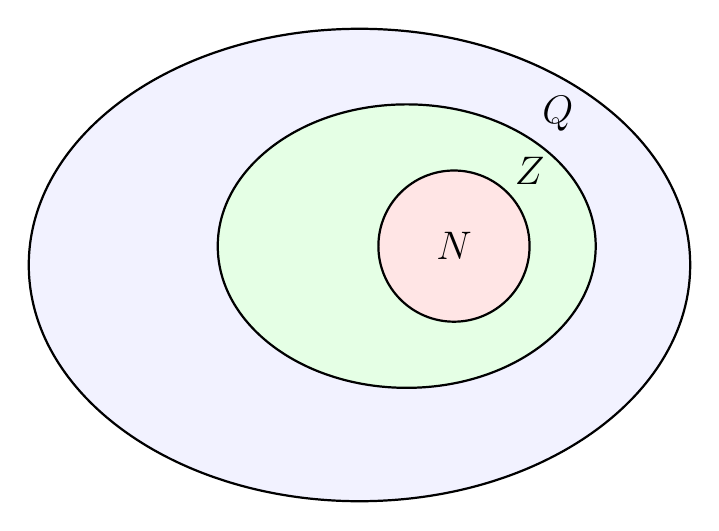
\begin{tikzpicture}[scale=1.2]
    % Elipse Q
    \draw[fill=blue!5,thick] (0,0) ellipse (3.5cm and 2.5cm);
    \node[font=\Large] at (2.1, 1.6) {\(\mathbb{Q}\)};
    
    % Elipse Z
    \draw[fill=green!10,thick] (0.5,0.2) ellipse (2cm and 1.5cm);
    \node[font=\Large] at (1.8, 1.0) {\(\mathbb{Z}\)};
    
    % Elipse N
    \draw[fill=red!10,thick] (1,0.2) ellipse (0.8cm and 0.8cm);
    \node[font=\Large] at (1, 0.2) {\(\mathbb{N}\)};
  \end{tikzpicture}
  \caption{Los números naturales están contenidos en los enteros, y los enteros están contenidos en los racionales.}
  \label{fig:jerarquia_numeros}
\end{figure}

Recuerde que la escritura decimal no constituye un nuevo conjunto numérico. Por ejemplo,
\[
0{,}5=\frac12
\]
por lo que \(0{,}5\) es un número racional.


\section[Práctica con racionales y división]{Ejercicios con productos, números racionales y división}

En los siguientes ejercicios utilizaremos conjuntamente las ideas desarrolladas en la segunda parte del capítulo. Conviene distinguir siempre entre el número representado y la forma particular utilizada para escribirlo. Una fracción, una división y una escritura decimal pueden, en ciertos casos, representar exactamente la misma cantidad.

\subsection*{Producto de números enteros}

Antes de evaluar cada producto, indique si el resultado será positivo, negativo o cero. Luego encuentre su valor.

\begin{enumerate}
\item \((-3)\cdot4\)
\item \(5\cdot(-2)\)
\item \((-6)\cdot(-3)\)
\item \((-7)\cdot1\)
\item \((-8)\cdot0\)
\item \((-1)\cdot12\)
\item \((-4)\cdot(-5)\)
\item \(9\cdot(-6)\)
\item \((-2)\cdot3\cdot4\)
\item \((-2)\cdot(-3)\cdot5\)
\item \((-1)\cdot(-1)\cdot(-1)\)
\item \((-4)\cdot2\cdot(-3)\)
\end{enumerate}

\subsection*{Completar productos con enteros}

Complete los espacios con un número entero que haga verdadera cada igualdad.

\begin{enumerate}
\item \((-3)\cdot\square=-12\)
\item \(5\cdot\square=-20\)
\item \((-6)\cdot\square=18\)
\item \(\square\cdot(-4)=20\)
\item \((-7)\cdot\square=0\)
\item \((-1)\cdot\square=9\)
\item \((-3)\cdot(-5)=3\cdot\square\)
\item \(4\cdot(-6)=(-4)\cdot\square\)
\end{enumerate}

\subsection*{Representaciones fraccionarias equivalentes}

Complete los espacios de manera que las fracciones representen el mismo número racional.

\begin{enumerate}
\item \(\dfrac12=\dfrac{\square}{4}\)
\item \(\dfrac23=\dfrac{\square}{12}\)
\item \(\dfrac35=\dfrac{12}{\square}\)
\item \(\dfrac47=\dfrac{20}{\square}\)
\item \(\dfrac{-2}{3}=\dfrac{-8}{\square}\)
\item \(\dfrac56=\dfrac{\square}{30}\)
\item \(\dfrac{7}{10}=\dfrac{21}{\square}\)
\item \(\dfrac{-3}{4}=\dfrac{\square}{20}\)
\item \(3=\dfrac{\square}{5}\)
\item \(-2=\dfrac{\square}{7}\)
\end{enumerate}

Ahora escriba tres representaciones fraccionarias diferentes para cada uno de los siguientes números:
\[
\frac12,\qquad \frac34,\qquad -\frac25,\qquad 2.
\]

\subsection*{Reconocer números racionales}

Responda en cada caso y justifique brevemente utilizando la definición de número racional.

\begin{enumerate}
\item ¿Por qué \(5\) es un número racional aunque esté escrito como un entero?
\item ¿Por qué \(-3\) es un número racional?
\item ¿La expresión \(\frac{4}{0}\) representa un número racional? Explique.
\item ¿La expresión \(\frac{0}{7}\) representa un número racional? ¿Qué número representa?
\item Escriba \(8\) como una fracción cuyo denominador sea \(3\).
\item Escriba \(-5\) como una fracción cuyo denominador sea \(4\).
\end{enumerate}

\subsection*{Producto de números racionales}

Encuentre una fracción que represente el valor de cada producto. Puede reemplazar la fracción obtenida por una representación equivalente más sencilla cuando sea posible.

\begin{enumerate}
\item \(\dfrac12\cdot\dfrac34\)
\item \(\dfrac23\cdot\dfrac57\)
\item \(\dfrac35\cdot\dfrac{10}{9}\)
\item \(\dfrac47\cdot\dfrac{14}{3}\)
\item \(\dfrac{-2}{3}\cdot\dfrac54\)
\item \(\dfrac34\cdot\dfrac{-8}{5}\)
\item \(\dfrac{-5}{6}\cdot\dfrac{-3}{10}\)
\item \(2\cdot\dfrac37\)
\item \((-4)\cdot\dfrac58\)
\item \(\dfrac79\cdot0\)
\item \(\dfrac{11}{5}\cdot1\)
\item \(\dfrac23\cdot\dfrac34\cdot\dfrac56\)
\end{enumerate}

\subsection*{Inversos multiplicativos}

Escriba el inverso multiplicativo de cada número, cuando exista.

\begin{enumerate}
\item \(\dfrac23\)
\item \(\dfrac57\)
\item \(-\dfrac34\)
\item \(4\)
\item \(-6\)
\item \(\dfrac{1}{9}\)
\item \(-1\)
\item \(1\)
\item \(\dfrac{-7}{2}\)
\item \(0\)
\end{enumerate}

En cada caso en que exista un inverso, compruebe su respuesta multiplicando ambos números y verificando que el resultado sea \(1\). En el caso de \(0\), explique por qué esa comprobación no puede realizarse.

\subsection*{Reescribir divisiones como productos}

Reescriba cada división como un producto por el inverso multiplicativo del divisor. No es necesario evaluarla todavía.

\begin{enumerate}
\item \(8\div2\)
\item \(5\div3\)
\item \((-6)\div2\)
\item \(7\div(-4)\)
\item \(\dfrac34\div2\)
\item \(\dfrac25\div\dfrac37\)
\item \(\dfrac{-4}{9}\div\dfrac23\)
\item \(3\div\dfrac58\)
\item \((-2)\div\dfrac{-7}{3}\)
\item \(\dfrac56\div(-5)\)
\end{enumerate}

Por ejemplo,
\[
\frac34\div\frac25
=
\frac34\cdot\frac52.
\]
La segunda expresión no representa una operación diferente: representa la misma división escrita mediante la definición \(x\div y=x\cdot y^{-1}\).

\subsection*{Evaluar divisiones}

Encuentre una fracción que represente el valor de cada expresión.

\begin{enumerate}
\item \(8\div2\)
\item \(15\div3\)
\item \(7\div4\)
\item \(1\div2\)
\item \((-12)\div3\)
\item \(18\div(-6)\)
\item \((-20)\div(-5)\)
\item \(\dfrac34\div\dfrac25\)
\item \(\dfrac56\div\dfrac23\)
\item \(\dfrac{-2}{7}\div\dfrac35\)
\item \(\dfrac49\div\dfrac{-8}{3}\)
\item \(2\div\dfrac37\)
\item \((-5)\div\dfrac{10}{3}\)
\item \(\dfrac78\div2\)
\item \(\dfrac32\div\dfrac94\)
\end{enumerate}

\subsection*{Completar igualdades con productos y divisiones}

Complete cada espacio con un número racional que haga verdadera la igualdad.

\begin{enumerate}
\item \(2\cdot\square=1\)
\item \(5\cdot\square=1\)
\item \((-4)\cdot\square=1\)
\item \(\dfrac37\cdot\square=1\)
\item \(\dfrac{-5}{2}\cdot\square=1\)
\item \(\square\div2=3\)
\item \(8\div\square=4\)
\item \(\dfrac34\div\square=\dfrac32\)
\item \(\square\div\dfrac25=\dfrac32\)
\item \(\dfrac56\cdot\square=\dfrac{5}{12}\)
\end{enumerate}

Observe que algunos de estos ejercicios pueden interpretarse como ecuaciones multiplicativas. Utilice la idea de inverso multiplicativo para justificar sus respuestas cuando resulte conveniente.

\subsection*{Restas sucesivas}

Utilice restas sucesivas para evaluar las siguientes divisiones. En cada caso, indique qué representa la cantidad de restas realizadas.

\begin{enumerate}
\item \(8\div2\)
\item \(12\div3\)
\item \(20\div4\)
\item \(18\div6\)
\item \(35\div5\)
\item \(42\div7\)
\end{enumerate}

Luego responda: ¿por qué este procedimiento no resulta suficiente para explicar directamente una división como \(1\div2\)?

\subsection*{Fracciones y escritura decimal}

Escriba cada fracción mediante una escritura decimal equivalente.

\begin{enumerate}
\item \(\dfrac{1}{10}\)
\item \(\dfrac{3}{10}\)
\item \(\dfrac{7}{10}\)
\item \(\dfrac{25}{100}\)
\item \(\dfrac{3}{4}\)
\item \(\dfrac12\)
\item \(\dfrac{5}{2}\)
\item \(\dfrac{7}{4}\)
\item \(\dfrac{15}{20}\)
\item \(\dfrac{125}{100}\)
\end{enumerate}

Ahora realice el proceso contrario: escriba cada número decimal como una fracción de enteros con denominador distinto de cero.

\begin{enumerate}
\item \(0{,}1\)
\item \(0{,}5\)
\item \(0{,}25\)
\item \(0{,}7\)
\item \(0{,}75\)
\item \(1{,}5\)
\item \(1{,}25\)
\item \(2{,}5\)
\item \(0{,}04\)
\item \(3{,}125\)
\end{enumerate}

\subsection*{Distintas representaciones del mismo número}

Complete los espacios de manera que todas las expresiones de cada fila representen el mismo número racional.

\begin{enumerate}
\item \(1\div2=\dfrac{\square}{2}=0{,}5\)
\item \(1\div4=\dfrac14=\square\)
\item \(3\div4=\dfrac34=\square\)
\item \(5\div2=\dfrac52=\square\)
\item \(7\div4=\dfrac74=\square\)
\item \(\dfrac{25}{100}=\dfrac{\square}{4}=0{,}25\)
\item \(0{,}5=\dfrac{5}{\square}=\dfrac12\)
\item \(1{,}25=\dfrac{125}{\square}=\dfrac54\)
\end{enumerate}

En estos ejercicios no aparecen números diferentes en cada miembro. Se muestran escrituras distintas de una misma cantidad.

\subsection*{Algoritmo de la división}

Utilice el algoritmo de la división o una descomposición equivalente basada en múltiplos del divisor. Muestre los pasos principales.

\begin{enumerate}
\item \(84\div7\)
\item \(96\div8\)
\item \(144\div12\)
\item \(156\div12\)
\item \(225\div15\)
\item \(324\div18\)
\item \(1\div2\)
\item \(3\div4\)
\item \(7\div4\)
\item \(9\div8\)
\end{enumerate}

En los casos en que el cociente no sea entero, continúe trabajando con décimos, centésimos o milésimos según resulte necesario.

\subsection*{Pertenencia a conjuntos numéricos}

Indique con una cruz (\(\times\)) a cuáles de los conjuntos \(\mathbb N\), \(\mathbb Z\) y \(\mathbb Q\) pertenece cada número. Un mismo número puede pertenecer a más de un conjunto.

\begin{center}
\begin{tabular}{c|c|c|c}
Número & Natural (\({N}\)) & Entero (\(Z\)) & Racional (\(Q\)) \\ \hline
\(10\) & & & \\ \hline
\(-7\) & & & \\ \hline
\(0\) & & & \\ \hline
\(3/4\) & & & \\ \hline
\(-5/2\) & & & \\ \hline
\(5{,}0\) & & & \\ \hline
\(0{,}5\) & & & \\ \hline
\(12/3\) & & & \\ \hline
\(-8/4\) & & & \\ \hline
\(0/9\) & & & \\ \hline
\(1{,}25\) & & & \\ \hline
\(-3{,}0\) & & &  
\end{tabular}
\end{center}

En los casos en que la escritura pueda ocultar el conjunto más pequeño al que pertenece el número, evalúe o reescriba primero la expresión. Por ejemplo, una fracción puede representar un entero.

\subsection*{Preguntas conceptuales}

Responda con una explicación breve. Cuando sea posible, acompañe su respuesta con una igualdad o con un ejemplo.

\begin{enumerate}
\item ¿Qué diferencia hay entre los factores de un producto y los sumandos de una suma?
\item ¿Por qué \(a\cdot0=0\) para cualquier número \(a\)?
\item ¿Por qué el producto por \(1\) no modifica el número representado?
\item ¿Por qué \((-a)\cdot(-b)=a\cdot b\)? Relacione su respuesta con la idea de opuesto.
\item ¿Por qué una misma cantidad racional puede escribirse mediante fracciones diferentes?
\item ¿Por qué el denominador de una fracción racional no puede ser cero?
\item ¿Por qué \(0\) no posee inverso multiplicativo?
\item ¿Qué significa afirmar que dividir por un número no nulo equivale a multiplicar por su inverso?
\item Explique por qué \(1\div2\), \(\frac12\) y \(0{,}5\) representan el mismo número.
\item ¿Por qué las restas sucesivas son una estrategia útil para algunas divisiones, pero no una definición general de la división?
\item ¿La escritura decimal crea un conjunto numérico nuevo? Justifique con un ejemplo del capítulo.
\item Explique con sus palabras la relación \(\mathbb N\subseteq\mathbb Z\subseteq\mathbb Q\).
\end{enumerate}

\subsection*{Construir expresiones}

Construya una expresión que cumpla cada condición. En muchos casos existen varias respuestas correctas.

\begin{enumerate}
\item Un producto de dos naturales que represente \(24\).
\item Dos productos diferentes que representen el mismo número natural.
\item Un producto de dos enteros negativos que represente \(30\).
\item Un producto de dos enteros cuyo resultado sea \(-24\).
\item Una fracción diferente de \(\frac12\) que represente el mismo número.
\item Dos fracciones diferentes que representen \(-\frac34\).
\item Un producto de dos racionales que represente \(1\), sin utilizar \(1\) como factor.
\item Una división cuyo resultado sea \(\frac12\).
\item Una división entre dos enteros cuyo resultado no sea entero.
\item Tres escrituras diferentes que representen \(0{,}5\).
\item Un número que pertenezca a \(\mathbb Q\) pero no a \(\mathbb Z\).
\item Un número que pertenezca a \(\mathbb Z\) pero no a \(\mathbb N\).
\end{enumerate}
